% Created 2020-12-23 Wed 13:09
% Intended LaTeX compiler: xelatex
\documentclass[12pt]{article}
\usepackage{graphicx}
\usepackage{grffile}
\usepackage{longtable}
\usepackage{wrapfig}
\usepackage{rotating}
\usepackage[normalem]{ulem}
\usepackage{amsmath}
\usepackage{textcomp}
\usepackage{amssymb}
\usepackage{capt-of}
\usepackage{hyperref}
\usepackage{minted}
\usepackage{amsmath}
\usepackage{amssymb}
\usepackage{setspace}
\usepackage{subcaption}
\usepackage{mathtools}
\usepackage{xfrac}
\usepackage[margin=1.25in]{geometry}
\usepackage[utf8]{inputenc}
\usepackage{color}
\usepackage{epsf}
\usepackage{tikz}
\usepackage{graphicx}
\usepackage{pslatex}
\usepackage{hyperref}
\usepackage[adobe-utopia]{mathdesign}
\usepackage{helvet}
\renewcommand{\familydefault}{\sfdefault}
\usepackage{textgreek}
\renewcommand*{\textgreekfontmap}{%
{phv/*/*}{LGR/neohellenic/*/*}%
{*/b/n}{LGR/artemisia/b/n}%
{*/bx/n}{LGR/artemisia/bx/n}%
{*/*/n}{LGR/artemisia/m/n}%
{*/b/it}{LGR/artemisia/b/it}%
{*/bx/it}{LGR/artemisia/bx/it}%
{*/*/it}{LGR/artemisia/m/it}%
{*/b/sl}{LGR/artemisia/b/sl}%
{*/bx/sl}{LGR/artemisia/bx/sl}%
{*/*/sl}{LGR/artemisia/m/sl}%
{*/*/sc}{LGR/artemisia/m/sc}%
{*/*/sco}{LGR/artemisia/m/sco}%
}
\makeatletter
\newcommand*{\rom}[1]{\expandafter\@slowromancap\romannumeral #1@}
\makeatother
\DeclarePairedDelimiterX{\infdivx}[2]{(}{)}{%
#1\;\delimsize\|\;#2%
}
\newcommand{\infdiv}{D\infdivx}
\DeclarePairedDelimiter{\norm}{\lVert}{\rVert}
\def\Z{\mathbb Z}
\def\R{\mathbb R}
\def\C{\mathbb C}
\def\N{\mathbb N}
\def\Q{\mathbb Q}
\def\noi{\noindent}
\onehalfspace
\usemintedstyle{bw}
\author{Sandy Urazayev\thanks{University of Kansas (ctu@ku.edu)}}
\date{345; 12020 H.E.}
\title{Enhancing Low Resolution Images with Convolutional Neural Network\\\medskip
\large MATH 596}
\hypersetup{
 pdfauthor={Sandy Urazayev},
 pdftitle={Enhancing Low Resolution Images with Convolutional Neural Network},
 pdfkeywords={},
 pdfsubject={},
 pdfcreator={Emacs 28.0.50 (Org mode 9.3)}, 
 pdflang={English}}
\begin{document}

\maketitle
\begin{flushleft}
But since I knew now that I could hope for nothing of greater value than
frivolous pleasures, what point was there in denying myself of them?
\end{flushleft}

\begin{flushright}
-- M. Proust
\end{flushright}

\section*{Abstract}
\label{sec:orgac8a8bf}
We live in a rather boring world, full of inconsistencies and patterns that we
fit our lives into. We still love it and try to capture its best shades for safe
storing. Unfortunately, time goes and the sharpness of our pictures and data
speedily fades. My final project would revolve around digital media enhancement
and resolution improvement. We will build a convolutional neural network that
will be able to learn the relationship between lower and higher resolution images.

\section*{Introduction}
\label{sec:org0291d68}
As we know, all digital imagse have different dimensions, encodings, sharpness,
colors, etc. No matter what the combination is, the human perception is always the
tower property of any digital media. The technology of the past was severely limited.
For example, about 30 years ago, an average CRT monitor would have a resolution of
320x200, which is mere 64000 pixels. cite:crt Our current monitors have a resolution
of at least 1920x1080 (2073600 pixels) and the new standard now is 3840x2160
(8294400 pixels). However, as technology progresses, the old recorded data doesn't.

Our old pictures, images, films, and movies in lower resolution don't get automatically
"converted" into higher and better resolution media. As time progresses, the older
media starts to scale badly and pales in comparison with current media. We also do
understand that legacy has to be preserved. We have Criterion Collection, a whole
industry company based on old films restoration. And many other companios are primarily
focused on media restoration, such as images. However, the whole process is very manual
in its method, which is proving to be very expensive and slow. We can do better than
this.

This paper will focus on a way we can automate the procedure with a rather simple
neural network and a couple of interesting techniques, such as convolution layers.
Some of the work introduced here is inspired by a previous research done on super
resolution images. cite:shi2016realtime

\section*{Data Overview}
\label{sec:org66110f4}
Machine Learning researchers cannot stress enough the importance of the training and
validation data we use to fit our models. I have been researching the best ways to
collect data.

Firstly, I had an idea to scrape the google image search results and then take those
images, compress them, and use them as the basis for the data. This approach proved
to introduce a couple of unfortunate complications, such as ethical issues with our
datasets, image filtering, very varying dimensions of images, little pattern
correlation, etc.

To address the issues above, I will use ImageNet image databases,cite:imagenet which
is a carefully curated set of training images that have a set size and ethical issues
resolved. I will use one of their Berkeley image nodes that has in total 500 images.
Some examples from the set are shown below

  \begin{figure}[h!]
	\centering
	\begin{subfigure}[b]{0.24\textwidth}
		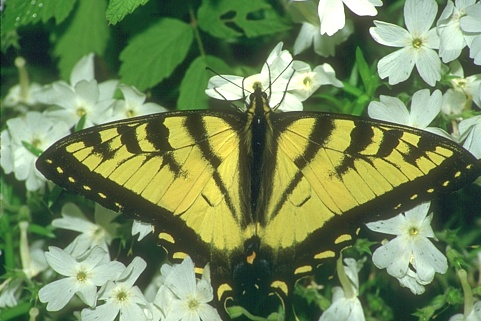
\includegraphics[width=\textwidth]{./1.jpg}
		\caption{First Sample}
		\label{fig:lenna37full}
	\end{subfigure}
	\hfill
	\begin{subfigure}[b]{0.24\textwidth}
		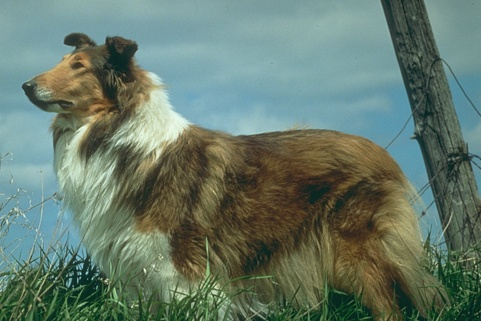
\includegraphics[width=\textwidth]{./2.jpg}
		\caption{Second Sample}
	\end{subfigure}
	\hfill
	\begin{subfigure}[b]{0.24\textwidth}
		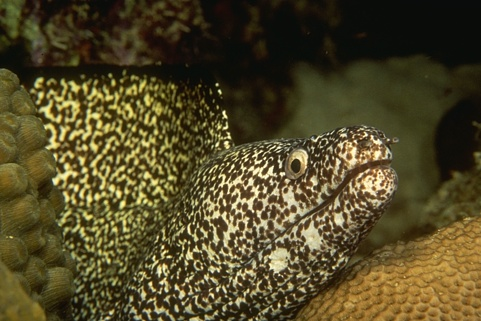
\includegraphics[width=\textwidth]{./3.jpg}
		\caption{Third Sample}
	\end{subfigure}
	\hfill
	\begin{subfigure}[b]{0.24\textwidth}
		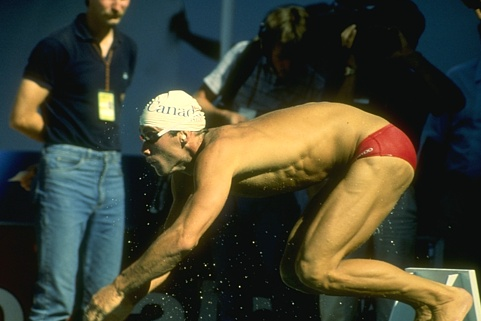
\includegraphics[width=\textwidth]{./4.jpg}
		\caption{Fourth Sample}
	\end{subfigure}
	\caption{ImageNet random samples}
\end{figure}

\section*{Design}
\label{sec:org07f2606}
Let's talk about how we would design the neural network to achieve our set goal. A
traditional neural network design would look the following way

\begin{figure}[h!]
	\centering
	\begin{subfigure}[b]{0.75\textwidth}
		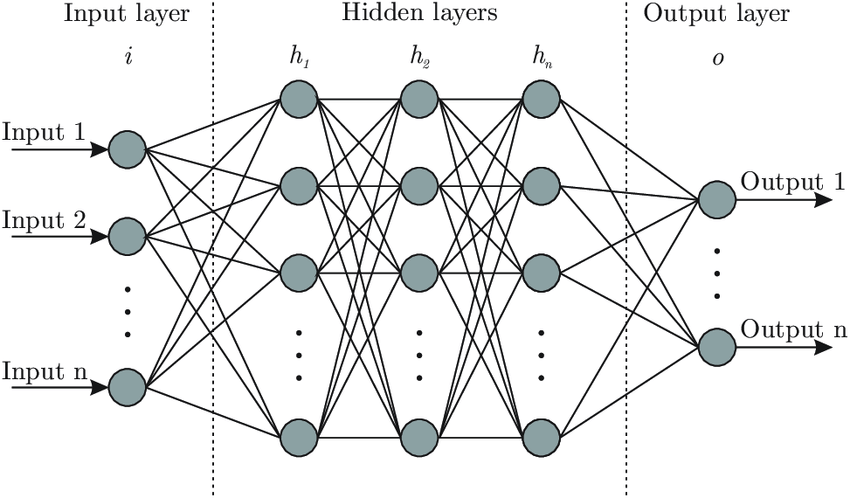
\includegraphics[width=\textwidth]{./nn.png}
	\end{subfigure}
	\caption{Traditional Neural Network}
\end{figure}

This has the same logic as our topics we learned in MATH 596. Neural Network is a
big distributed version of a multi-layered matrix. The learning process is the process
of filling up the values in our matrix and adjusting the weight of their connections,
so then patterns would emerge from input-output relationship. The difference from
convolutional neural network (CNN) is the application of milti-layered matrices in the
neural network schema itself, therefore it is more deeply involved when fitting the
training data. This of course increases the number of parameters we have to take care
of. However, this is still the best available machine learning technique we have for
computer vision applications. An example design of a CNN is below

\begin{figure}[h!]
	\centering
	\begin{subfigure}[b]{0.75\textwidth}
		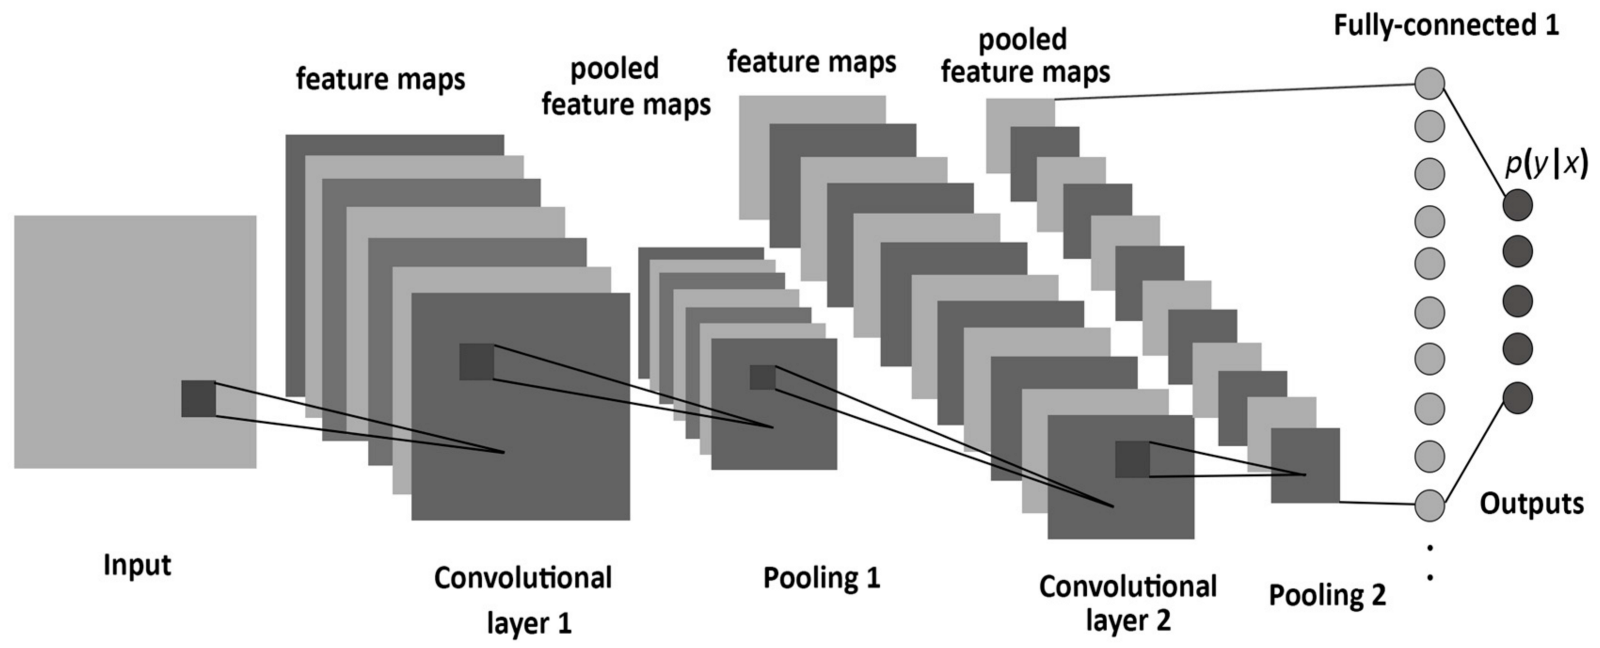
\includegraphics[width=\textwidth]{./cnn.png}
	\end{subfigure}
	\caption{Convolutional Neural Network}
\end{figure}

Multiple pooling layers are used to combine the pooled data from those convolution
layers.

\section*{Implementation}
\label{sec:orgc401cc5}
Our CNN implementation will be written in python using Tensorflow 2 and MacBook Pro M1
2020 hardware to train the model. First of all, we will define our input and output
dimensions, which are 100x100 and 300x300, respectively.

\begin{minted}[frame=lines,fontsize=\scriptsize,obeytabs,mathescape,numbersep=5pt,numbersep=2mm,xleftmargin=0.25in]{python}
# Basic input-output relationships
image_dimension = 300
scaling_factor = 3
input_dimension = image_dimension // scaling_factorp
\end{minted}

Next, let us define the way we will process the input and the output images. Regular
images have three layers: Red, Green, and Blue (RGB). However, running a training
triage on all three layers would be very heavy on our computational resources. We
will convert our images to YUV encoding, which would allow us to easily isolate the
brightness layer (luma component) and train our model on the grayscale version of the
image. Later on, just add on the other layers to complete the color gamma.

\begin{minted}[frame=lines,fontsize=\scriptsize,obeytabs,mathescape,numbersep=5pt,numbersep=2mm,xleftmargin=0.25in]{python}
def scale_image(image, _):
    return image / 255.0

def prepare_input(image, image_size, scaling):
    yuv = tf.image.rgb_to_yuv(image)
    y, u, v = tf.split(yuv, 3, axis=(len(yuv.shape) - 1))
    return tf.image.resize(y, [image_size, image_size],
                           method="area")

def prepare_output(image):
    yuv = tf.image.rgb_to_yuv(image)
    y, u, v = tf.split(yuv, 3, axis=(len(yuv.shape) - 1))
    return y

\end{minted}

\begin{itemize}
\item \texttt{scale\_image} simply scales each image color encoded value from \([0,255]\) to \([0,1]\).
This normalized version would ease off the burden of training.
\item \texttt{prepare\_input} simply resizes the image into the input requirements and extracts the
Y channel from an YUV encoding of our image.
\item \texttt{prepare\_output} prepares the output images by extracting the same Y channel as the
input layer.
\end{itemize}

Keras, our neural network training framewark has a great function call for us to embed
a whole training dataset with a single function call. Our training dataset and our
validation dataset are validated below

\begin{minted}[frame=lines,fontsize=\scriptsize,obeytabs,mathescape,numbersep=5pt,numbersep=2mm,xleftmargin=0.25in]{python}
train_directory = image_dataset_from_directory(
    images,
    batch_size=batch_size,
    image_size=(image_dimension, image_dimension),
    subset="training",
    validation_split=validation_split,
    seed=seed,
).map(scale_image)

validation_directory = image_dataset_from_directory(
    images,
    batch_size=batch_size,
    image_size=(image_dimension, image_dimension),
    subset="validation",
    validation_split=validation_split,
    seed=seed,
).map(scale_image)

\end{minted}

For this paper, we will select the 10\% of our whole dataset from ImageNet to be used
for validation and the remaining 90\% for training purposes.

Finally, let us get into the model structure. The beauty of convolution layers, is
that we have to carefully arrange them together and properly match their dimensions.
We will have a single input layer to accept 100x100 images, and 4 convolution layers,
with 64 neurons. 64 is chosen by fine-tuning. It's a natural heap size and works out
good!

\begin{minted}[frame=lines,fontsize=\scriptsize,obeytabs,mathescape,numbersep=5pt,numbersep=2mm,xleftmargin=0.25in]{python}
def build_model():
    layer_configs = {
        "activation": "relu",
        "kernel_initializer": "Orthogonal",
        "padding": "same",
    }

    input_layer = keras.Input(shape=(None, None, 1))
    x = layers.Conv2D(64, 5, **layer_configs)(input_layer)
    x = layers.Conv2D(64, 5, **layer_configs)(x)
    x = layers.Conv2D(64, 5, **layer_configs)(x)
    x = layers.Conv2D(scaling_factor ** 2, 3, **layer_configs)(x)
    output_layer = tf.nn.depth_to_space(x, scaling_factor)

    return keras.Model(input_layer, output_layer)


model = build_model()
model.summary()
\end{minted}

The resulting model is summarized as follows

\begin{verbatim}
_________________________________________________________________
Layer (type)                 Output Shape              Param #   
=================================================================
input_1 (InputLayer)         [(None, None, None, 1)]   0         
_________________________________________________________________
conv2d (Conv2D)              (None, None, None, 64)    1664      
_________________________________________________________________
conv2d_1 (Conv2D)            (None, None, None, 64)    102464    
_________________________________________________________________
conv2d_2 (Conv2D)            (None, None, None, 64)    102464    
_________________________________________________________________
conv2d_3 (Conv2D)            (None, None, None, 9)     5193      
_________________________________________________________________
tf.nn.depth_to_space (TFOpLa (None, None, None, 1)     0         
=================================================================
Total params: 211,785
Trainable params: 211,785
Non-trainable params: 0
\end{verbatim}

\section*{Mathematical Basis}
\label{sec:orgff29600}
Relu is a balancing function of the form \(\text{relu}(x) = \max\{0, x\}\) that will
activate only the neurons that really matter to the patterns we're studying. If a
connection on the weight bias is weak, relu will floor it to 0.

For our main optimization method, we will use a variance of Stochastic Optimization,
called Adam Algorithm. Adam optimization is a stochastic gradient descent method that
is based on adaptive estimation of first-order and second-order moments.

Convolutional Neural Networks incorporate all the topics we studied during this
semester. First of all, the optimization method, Adam optimization is a stochastic
gradient descent method that is trying to find the best approximations for global
minima, which are our errors. The greatest goal of any neural network is to minimize
the error of our model. We do that by trying to find the global minima of our error
space.

For error measurement, we will use a Peak signal-to-noise ratio (PSNR) error
approximation. It's similar to RMSE, with a couple of modifications that allow us
to apply it to differently-sized source and target matrices. Let \(I\) be our original
"ground-truth" image and \(K\) our approximation of the image.
Both have type \(\Z^{m \times m}\)
Then let \(MSE\) be

\begin{equation}
	MSE = \frac{1}{m^2} \sum_{i=0}^{m-1} \sum_{j=0}^{m-1} [I(i,j)-K(i,j)]^2
\end{equation}

then PSNR is defined as

\begin{equation}
	PSNR = 20 \times \log_{10}(MAX_I) - 10 \times \log_{10}(MSE)
\end{equation}

In this case, higher PSNR value means that the approximation is closer to the source.

\section*{Results}
\label{sec:orgeedd8d2}
\enlargethispage{\baselineskip}
The training for this model took about \textasciitilde{}2 hours just in 50 epochs and 450 images. The
better results would be achieved by training at least for 200 epochs with more than 100
thousand images. Let us review our results. I will use a matplotlib module for
enhancing a small part of the image's center to show the improvements the model can
bring.

Recall that a higher PSNR symbolizes a better approximation and the following test
images have never been seen by our model before. They are clean images pulled up from
untouched image datasets. The value in the captions is the PSNR against their respective
originals.

Notice that on average, the PSNR of our predictions are higher than the downscaled ones.
This is a firm confirmation that the sharpening works! Even a model with as little
training as this one, we were able to enhance an low resolution image with a
convolutional neural network.

\singlespace
\begin{figure}[h!]
  \centering
  \begin{subfigure}[b]{0.32\linewidth}
    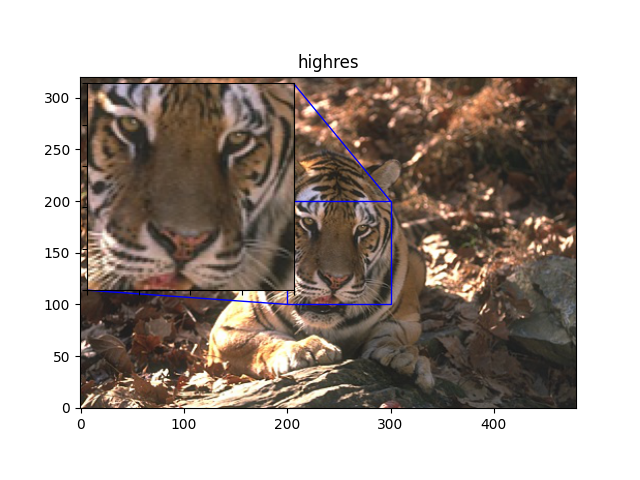
\includegraphics[width=\linewidth]{./0-highres.png}
    \caption{Original}
  \end{subfigure}
  \hfill
  \begin{subfigure}[b]{0.32\linewidth}
    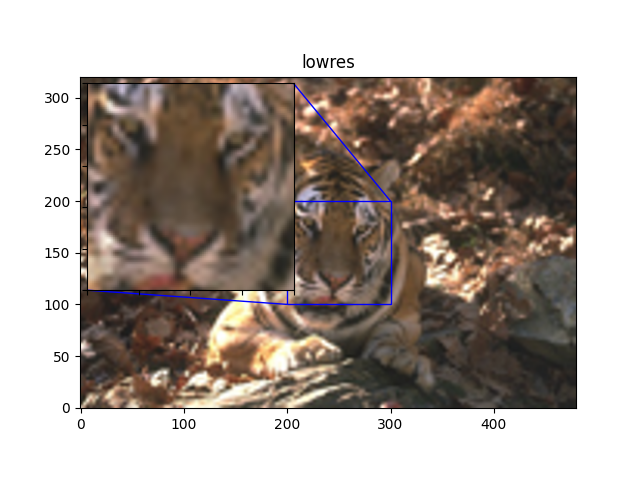
\includegraphics[width=\linewidth]{./0-lowres.png}
    \caption{Downscaled, 24.4263}
  \end{subfigure}
  \hfill
  \begin{subfigure}[b]{0.32\linewidth}
    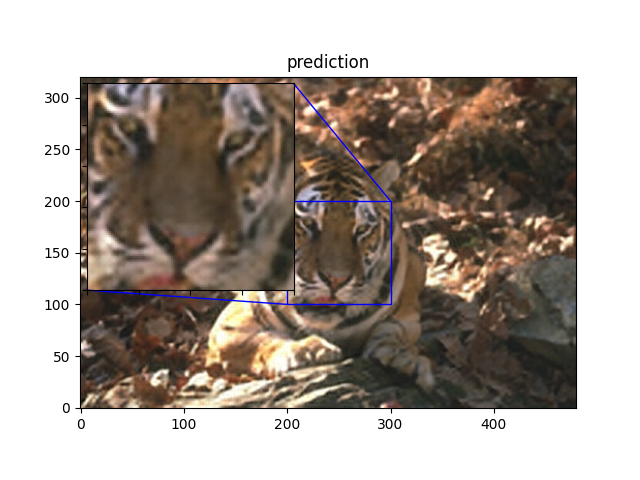
\includegraphics[width=\linewidth]{./0-prediction.png}
    \caption{Prediction, 25.3418}
  \end{subfigure}

  \begin{subfigure}[b]{0.32\linewidth}
    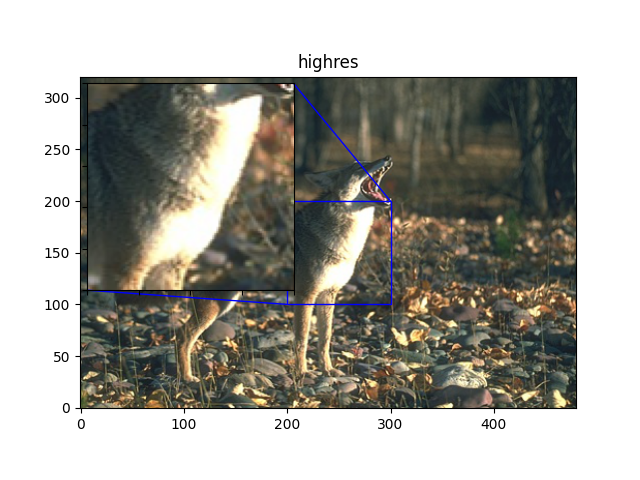
\includegraphics[width=\linewidth]{./1-highres.png}
    \caption{Original}
  \end{subfigure}
  \hfill
  \begin{subfigure}[b]{0.32\linewidth}
    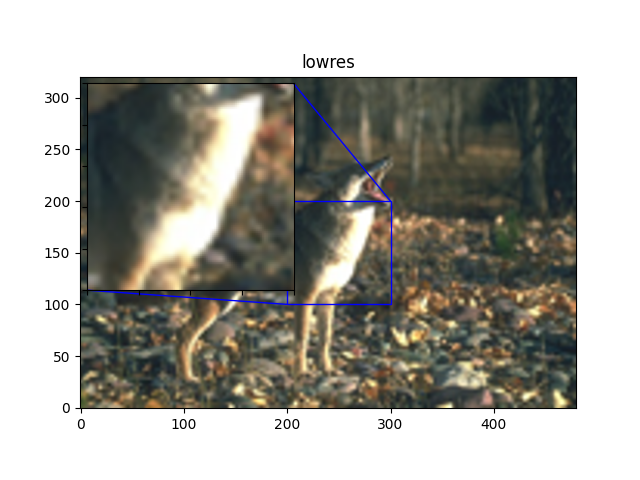
\includegraphics[width=\linewidth]{./1-lowres.png}
    \caption{Downscaled, 25.0398}
  \end{subfigure}
  \hfill
  \begin{subfigure}[b]{0.32\linewidth}
    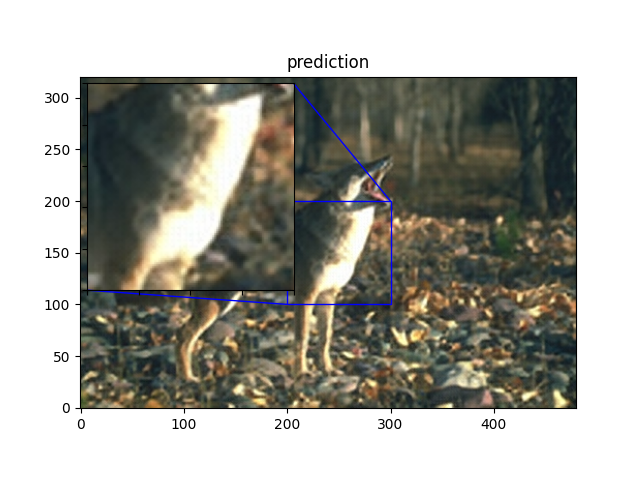
\includegraphics[width=\linewidth]{./1-prediction.png}
    \caption{Prediction, 25.6215}
  \end{subfigure}

  \begin{subfigure}[b]{0.32\linewidth}
    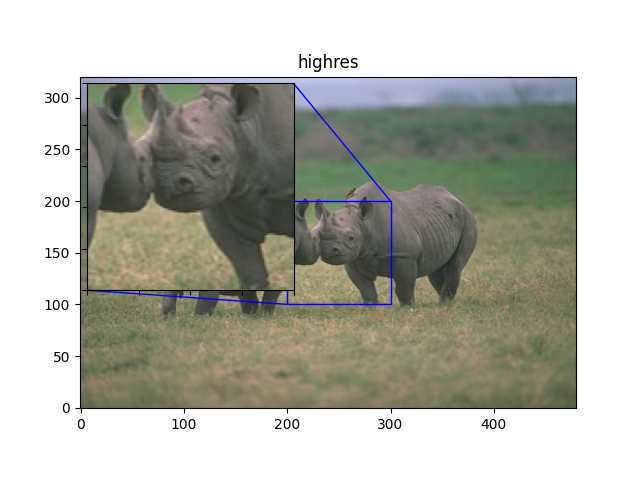
\includegraphics[width=\linewidth]{./2-highres.png}
    \caption{Original}
  \end{subfigure}
  \hfill
  \begin{subfigure}[b]{0.32\linewidth}
    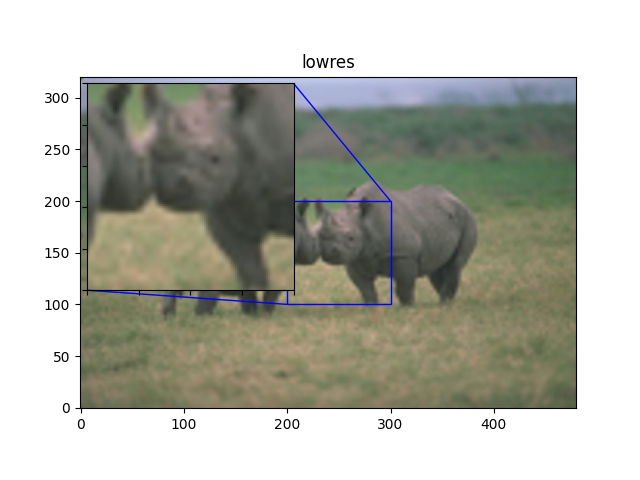
\includegraphics[width=\linewidth]{./2-lowres.png}
    \caption{Downscaled, 34.9506}
  \end{subfigure}
  \hfill
  \begin{subfigure}[b]{0.32\linewidth}
    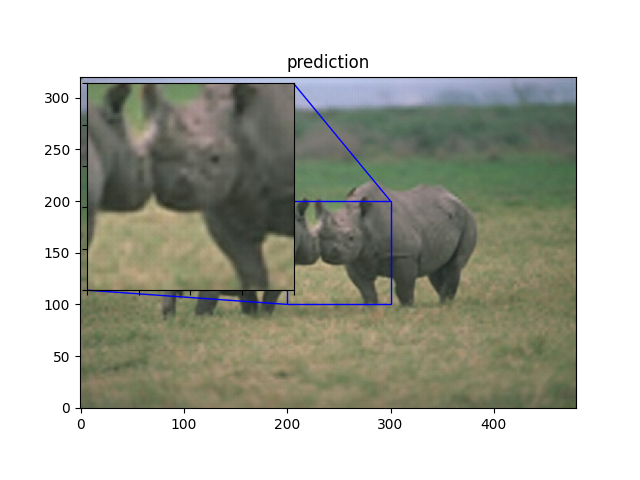
\includegraphics[width=\linewidth]{./2-prediction.png}
    \caption{Prediction, 34.9005}
  \end{subfigure}

  \begin{subfigure}[b]{0.32\linewidth}
    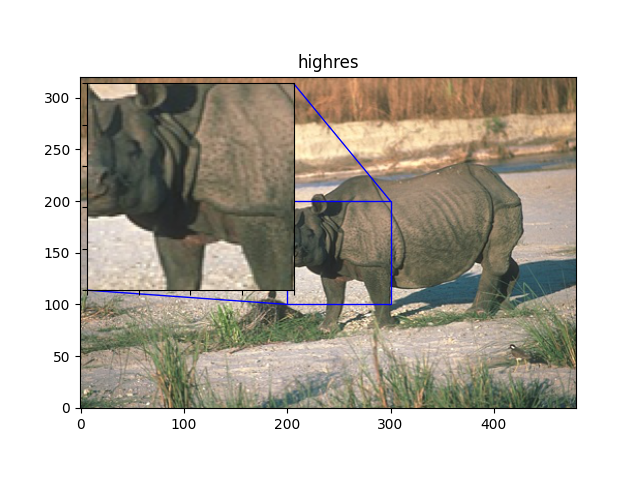
\includegraphics[width=\linewidth]{./3-highres.png}
    \caption{Original}
  \end{subfigure}
  \hfill
  \begin{subfigure}[b]{0.32\linewidth}
    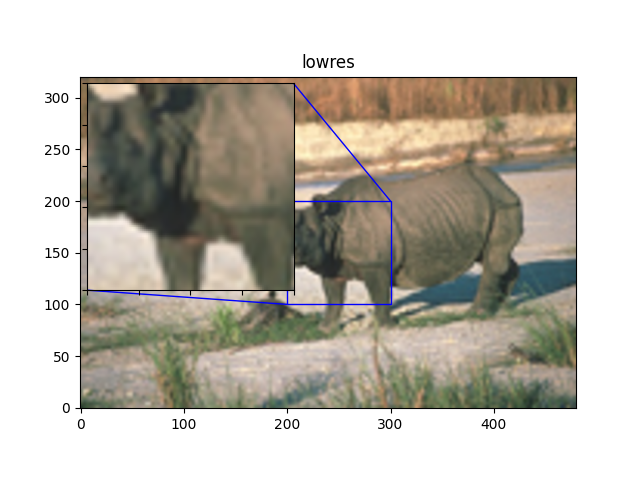
\includegraphics[width=\linewidth]{./3-lowres.png}
    \caption{Downscaled, 26.6250}
  \end{subfigure}
  \hfill
  \begin{subfigure}[b]{0.32\linewidth}
    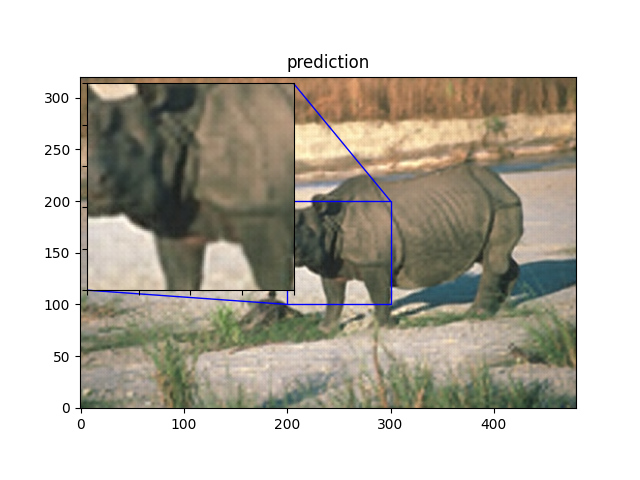
\includegraphics[width=\linewidth]{./3-prediction.png}
    \caption{Prediction, 27.0954}
  \end{subfigure}

  \begin{subfigure}[b]{0.32\linewidth}
    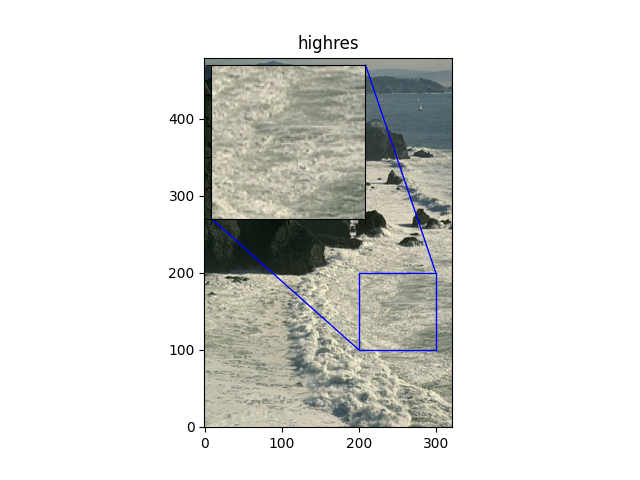
\includegraphics[width=\linewidth]{./4-highres.png}
    \caption{Original}
  \end{subfigure}
  \hfill
  \begin{subfigure}[b]{0.32\linewidth}
    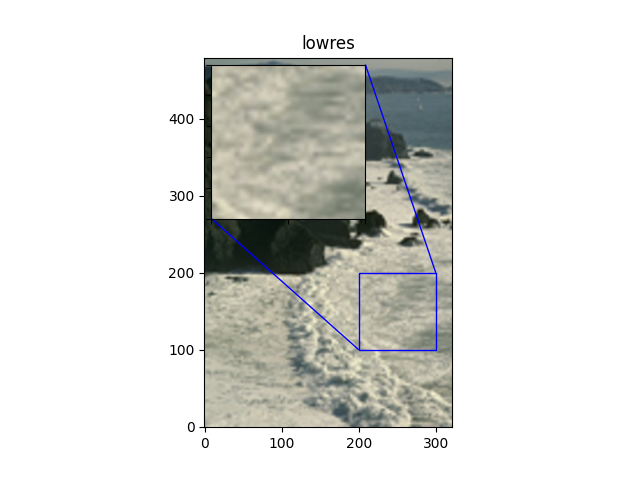
\includegraphics[width=\linewidth]{./4-lowres.png}
    \caption{Downscaled, 25.1637}
  \end{subfigure}
  \hfill
  \begin{subfigure}[b]{0.32\linewidth}
    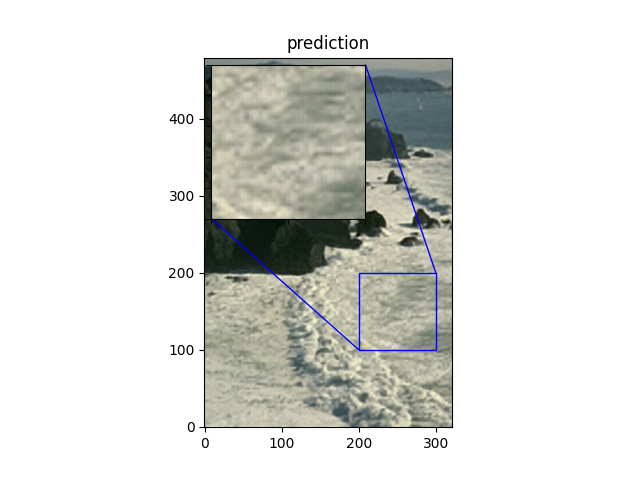
\includegraphics[width=\linewidth]{./4-prediction.png}
    \caption{Prediction, 25.5566}
  \end{subfigure}

\end{figure}

\begin{figure}[h!]
  \centering
  \begin{subfigure}[b]{0.32\linewidth}
    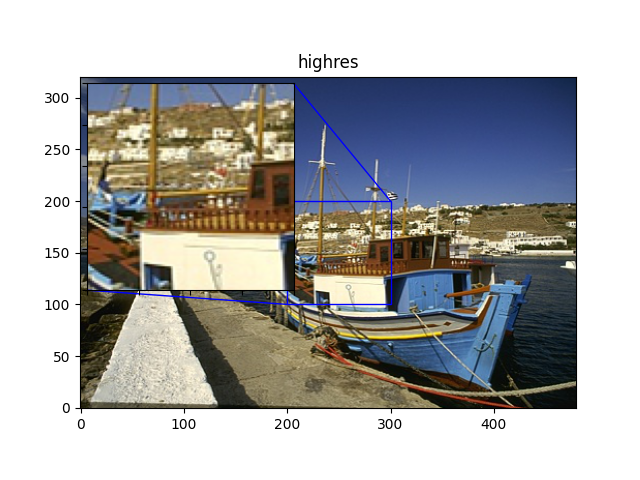
\includegraphics[width=\linewidth]{./5-highres.png}
    \caption{Original}
  \end{subfigure}
  \hfill
  \begin{subfigure}[b]{0.32\linewidth}
    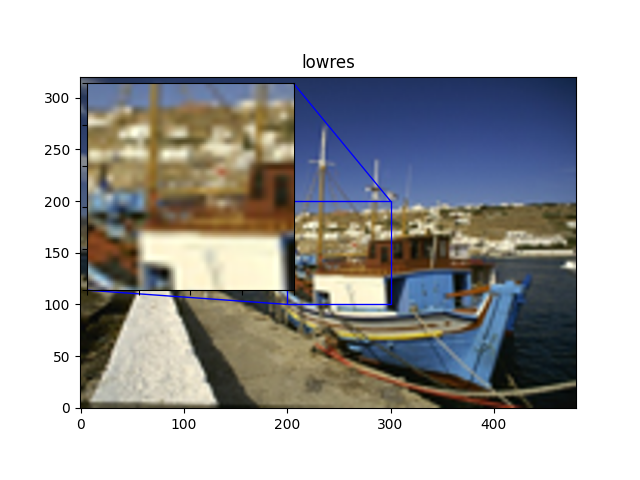
\includegraphics[width=\linewidth]{./5-lowres.png}
    \caption{Downscaled, 22.6681}
  \end{subfigure}
  \hfill
  \begin{subfigure}[b]{0.32\linewidth}
    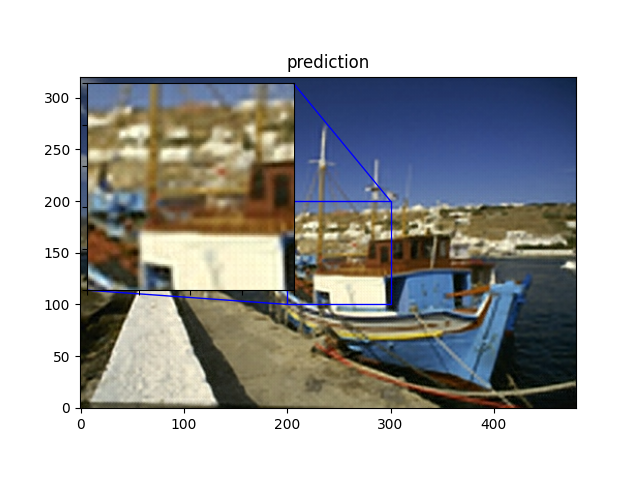
\includegraphics[width=\linewidth]{./5-prediction.png}
    \caption{Prediction, 23.2446}
  \end{subfigure}

  \begin{subfigure}[b]{0.32\linewidth}
    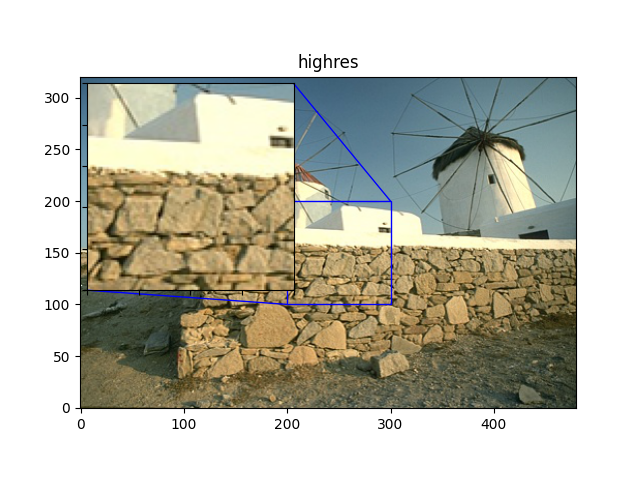
\includegraphics[width=\linewidth]{./6-highres.png}
    \caption{Original}
  \end{subfigure}
  \hfill
  \begin{subfigure}[b]{0.32\linewidth}
    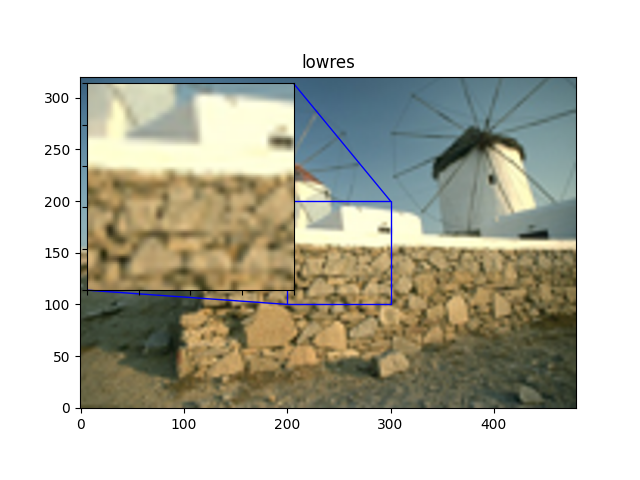
\includegraphics[width=\linewidth]{./6-lowres.png}
    \caption{Downscaled, 23.9902}
  \end{subfigure}
  \hfill
  \begin{subfigure}[b]{0.32\linewidth}
    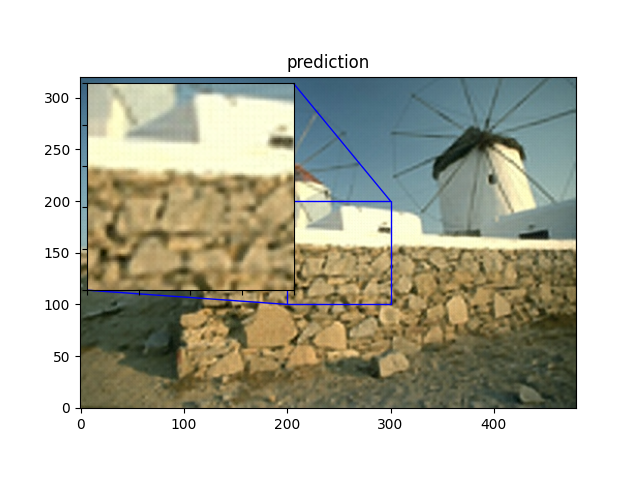
\includegraphics[width=\linewidth]{./6-prediction.png}
    \caption{Prediction, 24.4366}
  \end{subfigure}

  \begin{subfigure}[b]{0.32\linewidth}
    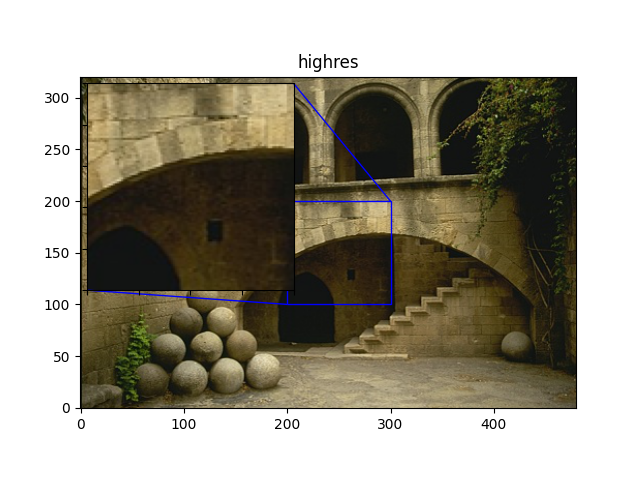
\includegraphics[width=\linewidth]{./7-highres.png}
    \caption{Original}
  \end{subfigure}
  \hfill
  \begin{subfigure}[b]{0.32\linewidth}
    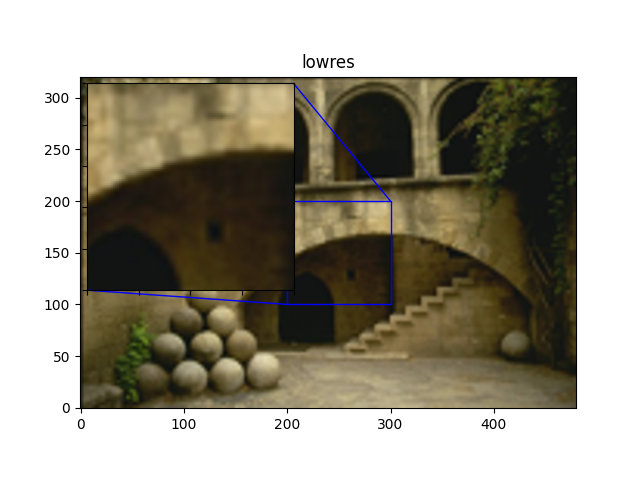
\includegraphics[width=\linewidth]{./7-lowres.png}
    \caption{Downscaled, 26.3472}
  \end{subfigure}
  \hfill
  \begin{subfigure}[b]{0.32\linewidth}
    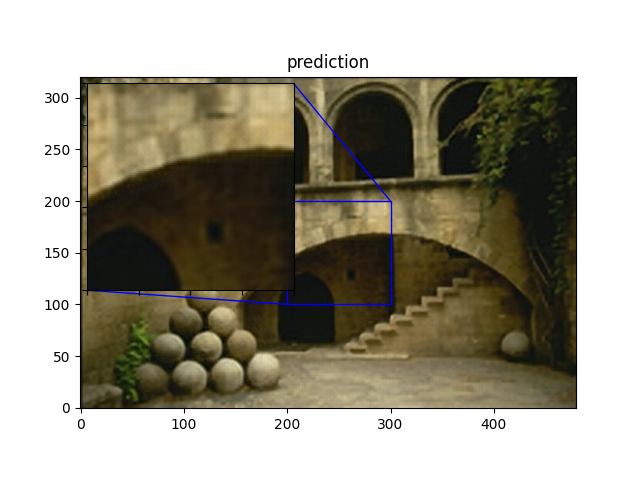
\includegraphics[width=\linewidth]{./7-prediction.png}
    \caption{Prediction, 26.8450}
  \end{subfigure}

  \begin{subfigure}[b]{0.32\linewidth}
    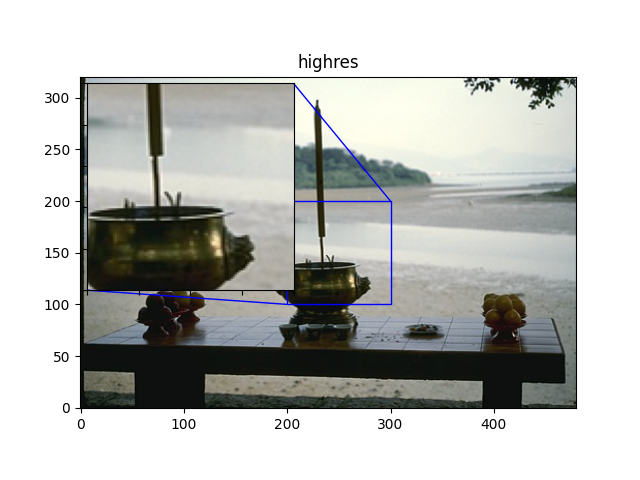
\includegraphics[width=\linewidth]{./8-highres.png}
    \caption{Original}
  \end{subfigure}
  \hfill
  \begin{subfigure}[b]{0.32\linewidth}
    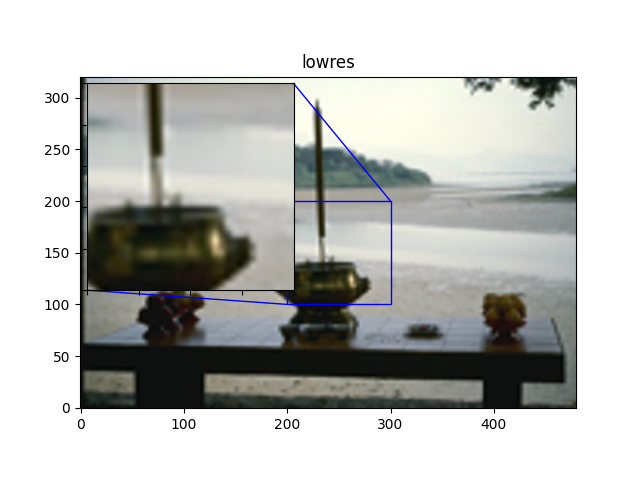
\includegraphics[width=\linewidth]{./8-lowres.png}
    \caption{Downscaled, 27.6660}
  \end{subfigure}
  \hfill
  \begin{subfigure}[b]{0.32\linewidth}
    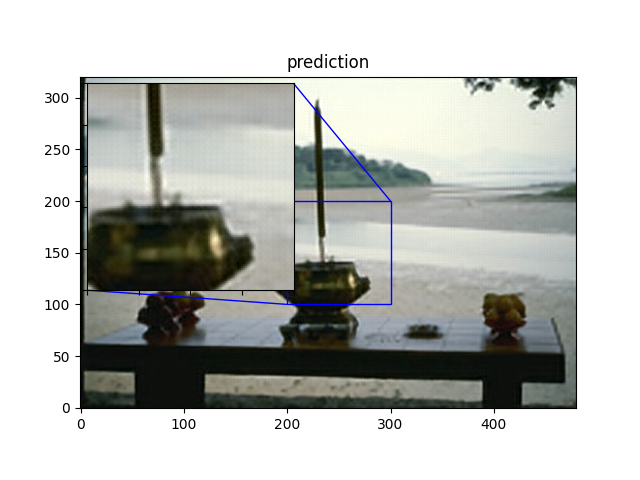
\includegraphics[width=\linewidth]{./8-prediction.png}
    \caption{Prediction, 29.0058}
  \end{subfigure}

  \begin{subfigure}[b]{0.32\linewidth}
    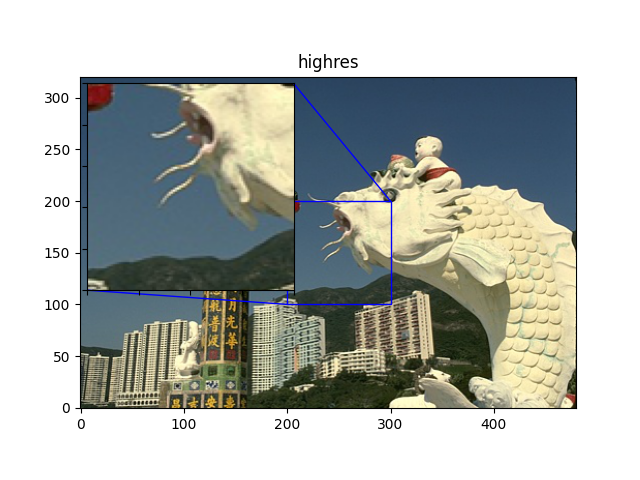
\includegraphics[width=\linewidth]{./9-highres.png}
    \caption{Original}
  \end{subfigure}
  \hfill
  \begin{subfigure}[b]{0.32\linewidth}
    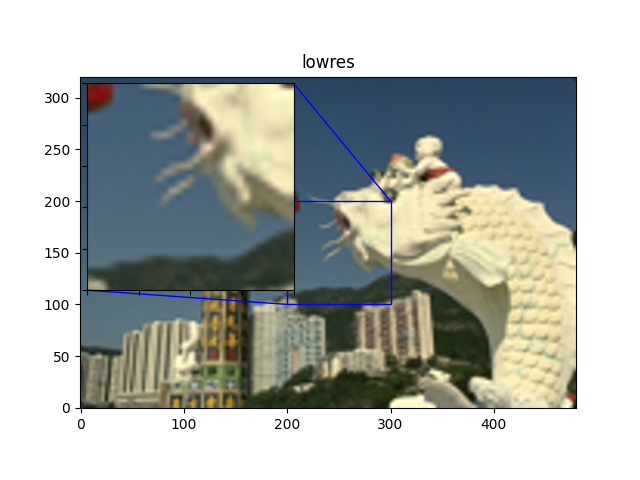
\includegraphics[width=\linewidth]{./9-lowres.png}
    \caption{Downscaled, 21.8129}
  \end{subfigure}
  \hfill
  \begin{subfigure}[b]{0.32\linewidth}
    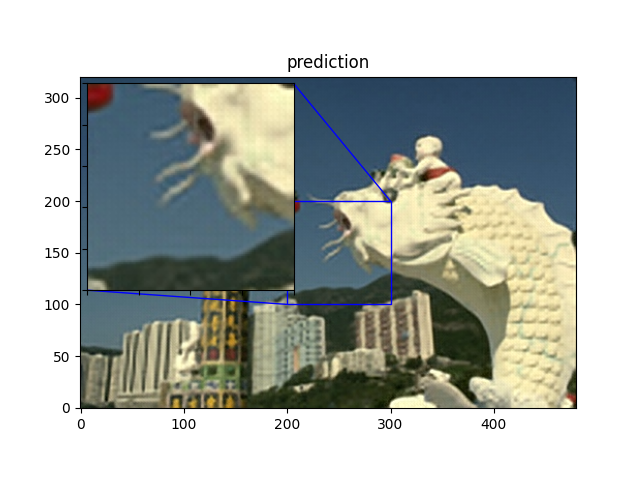
\includegraphics[width=\linewidth]{./9-prediction.png}
    \caption{Prediction, 22.2765}
  \end{subfigure}

\end{figure}        

bibliography:paper.bib
bibliographystyle:ieeetr
\end{document}
